\chapter{Balances Diferenciales}
Este capítulo consta de las siguientes partes:
\begin{enumerate}
	\item DIfusión en medios estacionarios.
	\item Difusión-Convección de masa.
	\item Difusión con reacción química homogénea.
	\item Difusión con reacción química hetereogénea.
	\item Difusión con reacción química en medios porosos.
\end{enumerate}

\section{Difusión en medios estacionarios}

\begin{figure}[H]
	\centering 
	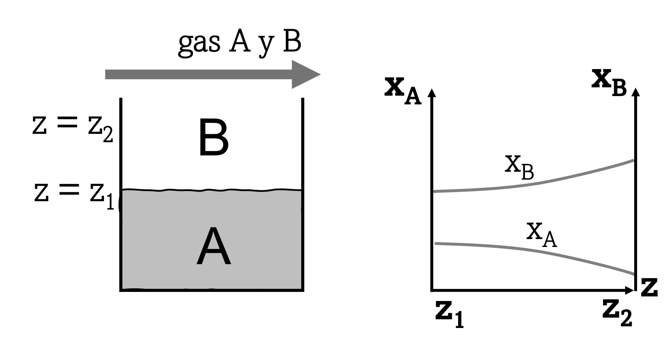
\includegraphics[scale=0.5]{./Capitulo2/Imagenes/fig-2-1.png}
	\caption{Columna de difusión. B no está en movimiento}
\end{figure}

A régimen permanente, la ec. (1.19) se reduce a:
\begin{equation}
\nabla \cdot \underline{N_A} = 0
\end{equation}

La ecuación (1.25) cuando $\underline{N_B} = 0$ se expresa como:

\begin{equation}
\underline{N_A} (1-x_A) = - c \mathcal{D}_{AB} \nabla x_A
\end{equation}

Si la difusión se da en una sola dirección (z), (2.1) y (2.2) requieren que:

\begin{equation}
	\frac{d}{dz} \left( \frac{c \mathcal{D}_{AB}}{1-x_A} \frac{dx_A}{dz} \right) = 0
\end{equation}

Integrando con respecto a z
$$
	\frac{1}{1-x_A} \frac{dx_A}{dz} = C_1
$$

Integrando de nuevo: 

\begin{equation}
- \ln{(1-x_A)} = C_1 z +C_2
\end{equation}

Condiciones de frontera 
\begin{equation}
	\left\{
	\begin{aligned}
	x_A |_{z=z_1} = x_{A1} \\
	x_A |_{z=z_2} = x_{A2}
	\end{aligned}
	\right.
\end{equation}

Se obtiene el siguiente perfil de concentraciones:

\begin{equation}
	\frac{1-x_A}{1-x_{A1}} = \left( \frac{1-x_{A2}}{1-x_{A1}} \right)^{\frac{z-z_1}{z_2-z_1}} 
	\qquad 
	1-x_A = x_B
\end{equation}

El flux de masa es:

\begin{equation}
N_{Az} |_{z=z_1} = \left. \frac{ - c \mathcal{D_{AB}}}{1-x_A} \frac{dx_A}{dz} \right|_{z=z_1} = \left. \frac{c \mathcal{D}_{AB}}{x_B} \frac{dx_B}{dz} \right|_{z=z_1} =  \frac{c \mathcal{D}_{AB}}{z_2 - z_1} \ln{\frac{x_{B2}}{x_{B1}}}
\end{equation}

que también puede ser expresado como: 

\begin{equation}
	N_{Az}|_{z=z_1} = \frac{c \mathcal{D}_{AB}}{(x_B)_{\ln{}}} \frac{(x_{A_1} - x_{A_2})}{z_2 - z_1}
\end{equation}

donde 

\begin{equation}
(x_B)_{\ln{}} = \frac{x_{B_2} - x_{B_1}}{\ln{(x_{B_2}/x_{B_1})}}
\end{equation}

En términos de las presiones, la ec. (2.8) se puede expresar: 

\begin{equation}
N_{Az}|_{z=z_1} = p \frac{\mathcal{D}_{AB}/RT}{z_2 - z_1} \ln{\left( \frac{p_{B_2}}{p_{B_1}}\right)} = p\frac{\mathcal{D}_{AB}/RT}{(p_B)_{\ln}} \frac{p_{A_1}-p_{A_2}}{z_2 - z_1}
\end{equation}


\subsection{Modelo de la película en transferencia de masa}

\begin{figure}[H]
	\centering
	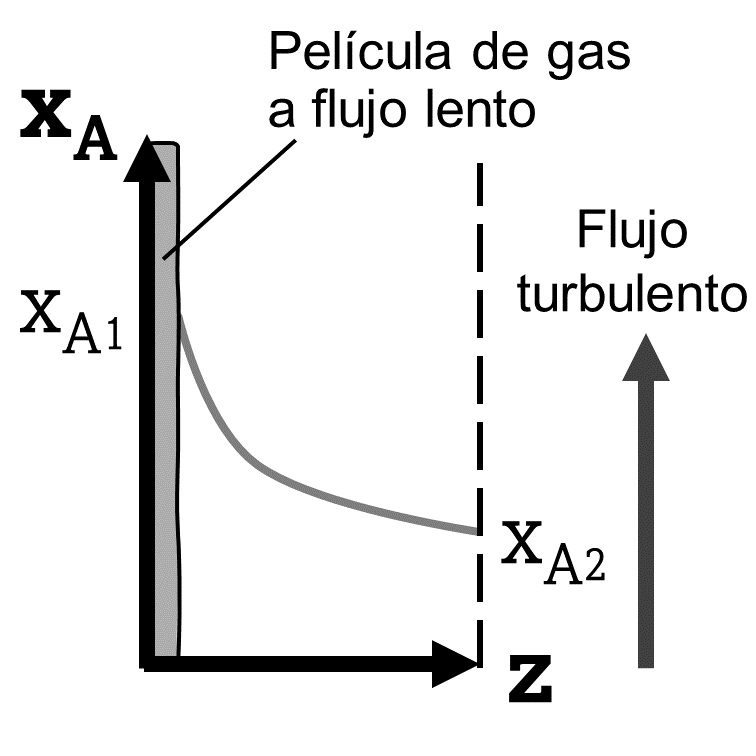
\includegraphics[scale=0.2]{./Capitulo2/Imagenes/fig-2-2.PNG}
	\caption{En este modelo, dentro de la película 		se produce la difusión de masa dentro de un 			medio a flujo lento.}
\end{figure}

\subsection{Difusión con interfase movible}

\begin{figure}[H]
	\centering
	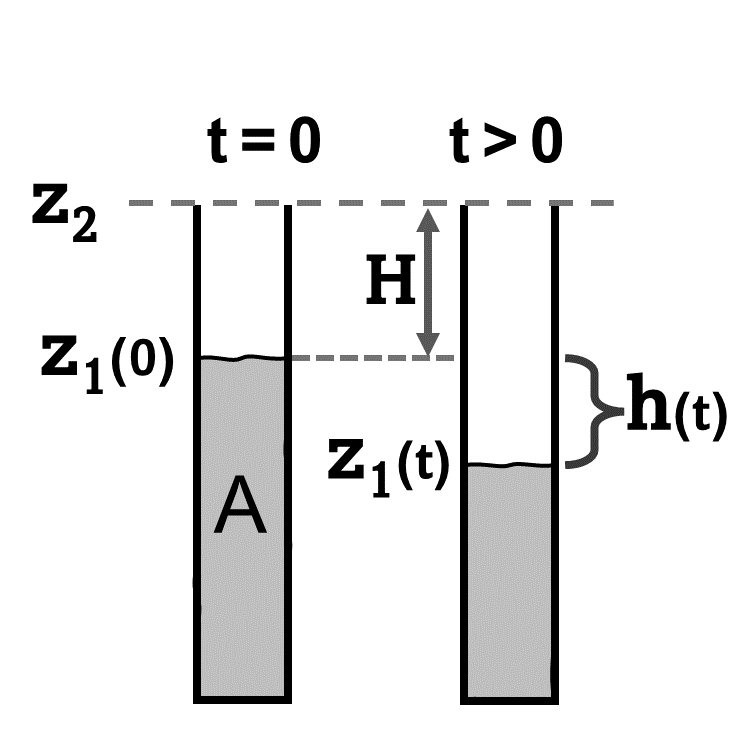
\includegraphics[scale=0.2]{./Capitulo2/Imagenes/fig-2-3.PNG}
	\caption{Evaporación con difusión cuasiestática. La mezcla de gases con concentración $x_{A_2}$ fluye arriba de los tubos.}
	\end{figure}
	
Primero, se iguala la velocidad de evaporación de $A$ con la velocidad a la que $A$ entra en la fase gas.

\begin{equation}
-\frac{p_A}{M_A} \frac{Sdz}{dt} = \frac{c \mathcal{D}_{AB}}{(x_B)_{\ln}} \frac{x_{A_1}-x_{A_2}}{z_2 - z_1} S
\end{equation}

Integrando la ec. (2.11): 

\begin{equation}
	\int_0^h (H+h)dh = \frac{c \mathcal{D}_{AB}}{(p_A/M_A)} \frac{(x_{A_1}-x_{A_2})}{(x_B)_{\ln}} \int_0^t dt = \frac{1}{2}c t
\end{equation}

en donde $h(t) = z_1(0) - z_1(t)$ y $H = z_2 - z_1(0)$ es la distancia inicial de la columna de gas. $c$ es una constante.

Integrando: 

\begin{equation}
	h(t) = H \left[ \sqrt{1+ct/H^2}-1 \right]
\end{equation}

Este experimento puede aportar la difusividad de mediciones del nivel del líquido como función del tiempo.

\subsection{Determinación de la difusividad}

La difusividad del par de gases $O_2 - CCl_4$ puede ser determinada por medio de datos de evaporación del $CCl_4$ en un tubo que contiene $O_2$ (ver figura 2.1). La distancia entre el nivel del $CCl_4$ líquido y la parte superior del tubo es $z_2 - z_1 = 17.1 \hspace{0.1cm} cm$. La presión total del sistema es $755 \hspace{0.1cm} mmHg$. y la temperatura es $0•^\circ C$. La presión de vapor del $CCl_4$ a $0•^\circ C$ es $33 \hspace{0.1cm} mmHg$. El área de sección del tubo es $0.82 \hspace{0.1cm} cm^2$. Se midieron $0.0208 \hspace{0.1cm} cm^3$ de $CCl_4$ evaporados en $10 \hspace{0.1cm} hrs$ en régimen permanente. ¿ Cuál es la difusividad del par $O_2 - CCl_4$ ?

\underline{Solución}:

Si $A=CCl_4$ y $B=O_2$. Entonces el flux molar de $A$ es:

$$N_A = \frac{\rho \text{Vol}}{M_A At} = \frac{(1.59)(0.0208)}{(154)(0.82)(36000)} = 7.26 \times 10­^{-9} gmol/cm^2 s$$ 

De la ec. (2.10):

$$N_{A_z} | _{z=z_1} = \frac{p}{RT} \mathcal{D}_{AB} \frac{\ln{(p_{B_2}/p_{B_1})}}{z_2 - z_1}$$

$$\mathcal{D}_{AB} = (7.2 \times 10^{-9})\frac{(17.1)}{\ln{(p_{B_2}/p_{B_1})}} \frac{RT}{p}$$

donde $R = 82.06 \hspace{0.1cm} \frac{cm^3 atm}{gmol K}$, $T = 273 \hspace{0.1cm} K$

$$p = \frac{755}{760} \hspace{0.1cm} atm , \hspace{0.5cm} \frac{p_{B_2}}{p_{B_1}} = \frac{755}{755-33}$$

$$\mathcal{D}_{AB} = 0.0636 \hspace{0.1cm} cm^2/s$$
	
\section{Difusión-Convección de masa}

\subsection{Convección forzada. Absorción de gas $A$ en una película descendente de líquido $B$}

\begin{figure}[H]
	\centering
	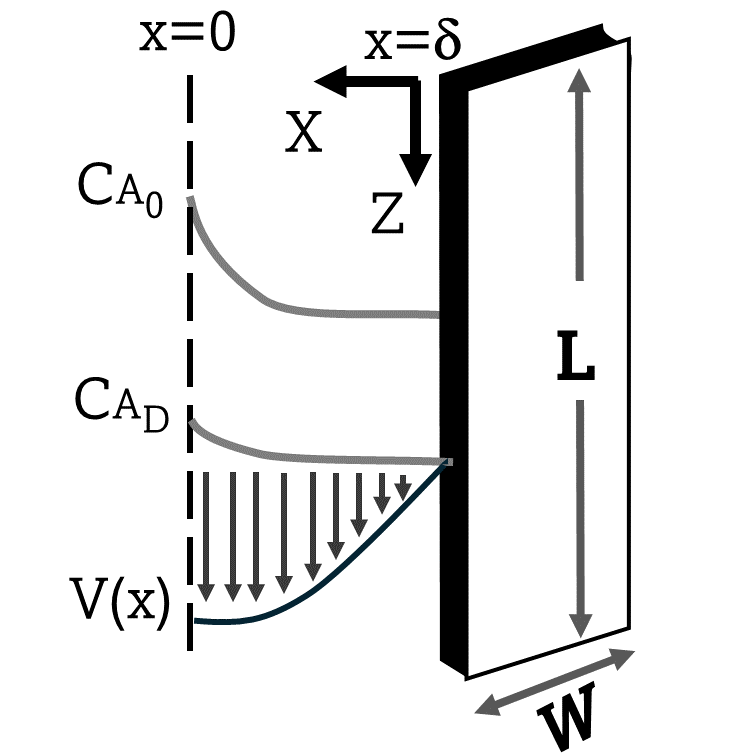
\includegraphics[scale=0.2]{./Capitulo2/Imagenes/fig-2-4.PNG}
	\caption{Absorción de $A$ en una película descendente de líquido $B$.}
\end{figure}

El perfil de velocidades en una solución diluida (la viscosidad es la del solvente) es:

\begin{equation}
v_z(x) = v_{\text{máx}} \left( 1 - \frac{x^2}{\delta^2} \right)
\end{equation}

Si el perfil de concentraciones se da en la zona de velocidad máxima, se puede considerar una velocidad constante $v_{\text{máx}}$. Un ejemplo es la absorción de $O_2$ en $H_2O$.

Debido a que $C_A = C_A(x,z)$, existen dos fluxes $N_{Ax}$ y $N_{Az}$. La ec. (2.1) a régimen permanente y sin reacción química se reduce a:

\begin{equation}
	\nabla \cdot \underline{N_A} = 0 \to \frac{\partial N_{Ax}}{\partial x} + \frac{\partial N_{Az}}{\partial z} = 0
\end{equation}

A partir de la ec. (1.30) se obtiene:

%\begin{equation}%
%Use \label{original} and \tag{\ref{eq:original}}%
$$	\underline{v} \cdot \nabla C_A = \mathcal{D}_{AB} \nabla^2 C_A $$
%\end{equation}%

que para $\underline{v} = (0, 0, v_z)$ tenemos:

\begin{equation} \label{eq: manrefx}
	v_z \frac{\partial C_A}{\partial z} = \mathcal{D}_{AB} \left[ \frac{\partial^2 C_A}{\partial x^2} + \frac{\partial^2 C_A}{\partial z^2}  \right]
\end{equation}

Definiendo al número de Peclet de masa ($Pe_M$) como: 

\begin{equation}
	Pe_M = Re Sch = \frac{uL}{\nu} \cdot \frac{\nu}{\mathcal{D}_{AB}} = \frac{uL}{\mathcal{D}_{AB}}
\end{equation}

donde $u$ y $L$ son la velocidad y longitud características. En este caso $u = v_{\text{máx}}$. Se supone que a lo largo del eje $z$:

$$Pe_M = \frac{v_{\text{máx}} L}{\mathcal{D}_{AB}} > 1$$

El término convectivo predomina sobre el difusivo, por lo que

$$v_z \frac{\partial C_A}{\partial z} > \mathcal{D}_{AB} \frac{\partial^2 C_A}{\partial z^2}$$

y la ec. \eqref{eq: manrefx} se simplifica:

\begin{equation} \label{eq: manrefx2}
v_{z \text{máx}} \frac{\partial C_A}{\partial z} = \mathcal{D}_{AB} \frac{\partial^2 C_A}{\partial x^2}
\end{equation}

Como $dt = \frac{dz}{v_{\text{máx}}}$, entonces la ec. \eqref{eq: manrefx2} se expresa como:

\begin{equation} \label{eq: manrefx3}
	\frac{\partial C_A}{\partial t} = \mathcal{D}_{AB} \frac{\partial^2 C_A}{\partial x^2}
\end{equation}

Las condiciones de frontera son:

\begin{equation}
	\text{Condición inicial:} \hspace{0.5cm} C_A|_{z=0} = 0 \hspace{0.5cm} \text{($B$ puro)}
\end{equation}

\begin{equation}
	 \text{Condición de interfase:} \hspace{0.4cm} C_A|_{x=0} = C_{A0} \hspace{0.4cm} \text{(Solubilidad de $A$ en $B$)}
\end{equation}

La condición $\left. \frac{\partial C_A}{\partial x} \right|_{x = \delta} = 0$ (flujo de masa es cero en la pared) se cambia por:

\begin{equation}
	C_A|_{x \to \infty} = 0
\end{equation}

(el perfil de $C_A$ se encuentra cerca de la interfase y lejos de la pared)

Considerando la concentración de $C_A$ adimensional:

\begin{equation}
	C_A' = \frac{C_A}{C_{A0}}
\end{equation}

La solución de \eqref{eq: manrefx3} se obtiene por el método de combinación de variables, que consiste en formar un grupo adimensional con las variables de la ecuación. Se sugiere la siguiente relación:

\begin{equation}
	C_A' = C_A'(\eta) \hspace{0.5cm} \text{donde} \hspace{0.5cm} \eta = \frac{x}{\sqrt{4 \mathcal{D}_{AB} t}}
\end{equation}

de tal forma que:

\begin{equation} \label{eq: manrefx4}
	\frac{d C_A'}{dt} = \frac{d C_A'}{d \eta} \frac{\partial \eta}{\partial t} = \frac{x}{\sqrt{4 \mathcal{D}_{AB}}} \left( - \frac{1}{2} t^{-3/2}  \right) = - \frac{1}{2} \frac{\eta}{t} \frac{d C_A'}{d \eta}
\end{equation}

$$\frac{dC_A'}{dx} = \frac{dC_A'}{d \eta} \frac{\partial \eta}{\partial x} = \frac{1}{\sqrt{4 \mathcal{D}_{AB} t}} \frac{dC_A'}{d \eta}$$

\begin{equation} \label{eq: manrefx5}
	\frac{\partial^2 C_A'}{\partial x^2} =  \frac{d^2 C_A'}{d \eta^2} \frac{1}{4 \mathcal{D}_{AB}t}
\end{equation}

Sustituyendo \eqref{eq: manrefx4} y \eqref{eq: manrefx5} en la ec. \eqref{eq: manrefx3} se obtiene: 

\begin{equation} \label{eq: manrefx6}
	\frac{d^2 C_A'}{d \eta^2} + 2\eta \frac{d C_A'}{d \eta} = 0
\end{equation}

Condiciones de frontera:

\begin{equation} \label{eq: manrefx7}
	C_A'|_{\eta = 0} = 1
\end{equation}

\begin{equation} \label{eq: manrefx8}
	C_A'|_{\eta \to \infty} = 0
\end{equation}

La primera integración de la ec. \eqref{eq: manrefx6} da:

Si $\frac{d C_A'}{d \eta} = \phi \to \frac{d\phi}{d \eta} + 2 \eta \phi = 0 \to \ln{\phi} = -\eta^2 + \ln{C_1}$

\begin{equation} \label{eq: manrefx8.1}
	\frac{dC_A'}{d \eta} = C_1 e^{-\eta^2}
\end{equation}

La segunda integración da por resultado:

\begin{equation} \label{eq: manrefx9}
	C_A' = C_1 \int_0^\eta e^{-\bar{\eta}^2} d\bar{\eta} + C_2
\end{equation}

La condición \eqref{eq: manrefx7} implica que $C_2 = 1$. La condición \eqref{eq: manrefx8} nos da:

$$0 = C_1 \int_0^\infty e^{-\bar{\eta}^2} d\bar{\eta} +1 = C_1 \frac{\sqrt{\pi}}{2} + 1 \to C_1 = \frac{-2}{\sqrt{\pi}}$$

Sustituyendo $C_1$ y $C_2$ en la ec. \eqref{eq: manrefx9} obtenemos: 

\begin{equation}
C_A' = 1 - \frac{2}{\sqrt{\pi}} \int_0^\eta e^{-\bar{\eta}^2} d\bar{\eta} = 1 - \text{erf} (\eta) = \text{erfc}(\eta) 
\tag{\ref{eq: manrefx8.1}}
\end{equation}

 donde $\text{erf} (\eta)$ es la función error y $\text{erfc}(\eta)$ es la función complementaria (ver fig. 2.5).
 
 \begin{figure}[H]
 	\centering
 	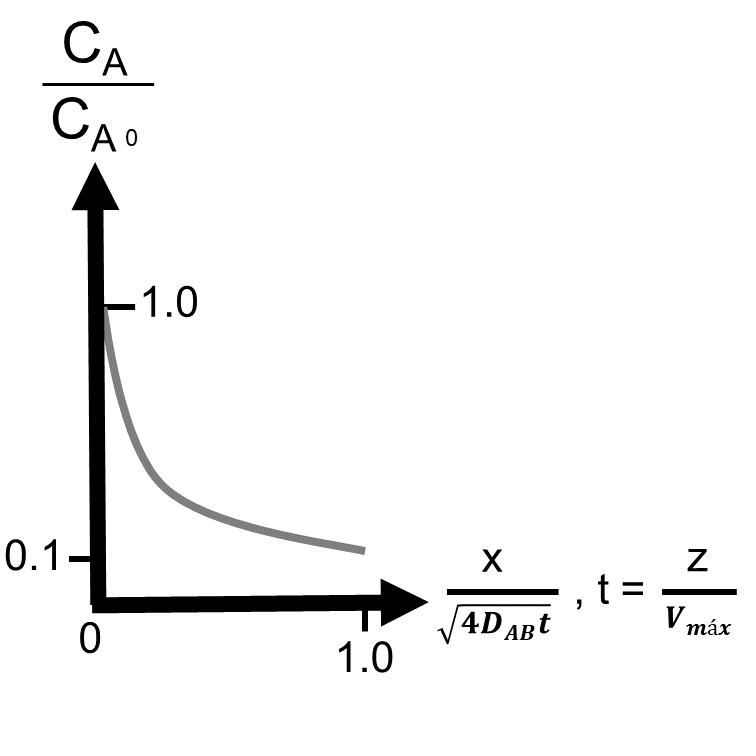
\includegraphics[scale=0.3]{./Capitulo2/Imagenes/fig-2-5.PNG}
 	\caption{Perfil de concentraciones donde $\delta$ es la longitud característica para la difusión de A en B.}
 \end{figure}
 
 Cuando $\eta = 2$, $\frac{C_A}{C_{A0}} \sim 0.01$ se puede definir una capa límite de difusión de $A$ en $B$ $\frac{\delta}{\sqrt{4\mathcal{D}_{AB}t}} = 2 \to \delta = 4 \sqrt{\mathcal{D}_{AB}t}$
 
 El flux de masa local en la interfase se puede obtener:
 
 $$N_{Ax}|_{x=0} = -\mathcal{D}_{AB} \left. \frac{\partial C_A}{\partial x} \right|_{x=0} = -\mathcal{D}_{AB} C_{A0} \left. \frac{\partial C_A'}{\partial \eta} \right| _{\eta = 0} \frac{\partial \eta}{\partial x} = -\mathcal{D}_{AB} \left( \frac{-2}{\sqrt{\pi}} \right) \frac{C_{A0}}{\sqrt{\mathcal{D}_{AB}t}}$$
 
 \begin{equation}
 	N_{Ax}|_{x=0} = C_{A0} \sqrt{\frac{\mathcal{D}_{AB}t}{\pi}} = C_{A0} \sqrt{ \frac{\mathcal{D}_{AB} v_{\text{máx}}}{\pi z}}
 	\tag{\ref{eq: manrefx9}}
 \end{equation}
 
 El flujo de masa de $A$ absorbido por $B$ es la superficie $LW$ es:
 
 $$W_A = \int_0^W \int_0^L N_{Ax}|_{x=0} dz dy = WC_{A0} \sqrt{\frac{\mathcal{D}_{AB} v_{\text{máx}}}{\pi}} \int_0^L \frac{dz}{\sqrt{z}}$$
 
 \begin{equation} \label{eq: manrefx10}
 W_A = WLC_{A0} \sqrt{\frac{4\mathcal{D}_{AB} v_{\text{máx}}}{\pi L}}
 \end{equation}
 
 Este desarrollo se puede aplicar a la absorción de gas en burbujas ascendentes.
 
 \begin{figure}[H]
 	\centering
 	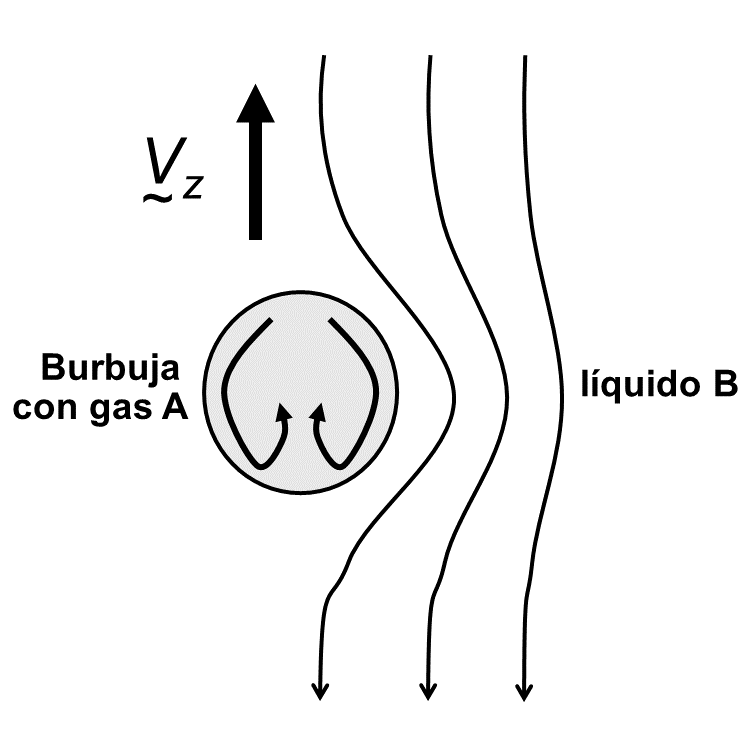
\includegraphics[scale=0.2]{./Capitulo2/Imagenes/fig-2-6.PNG}
 	\caption{Burbuja de gas $A$ ascendiendo en un líquido $B$ a velocidad $\underline{v_t}$.}
 \end{figure}
 
 Se puede utilizar la ec. \eqref{eq: manrefx10} para calcular la absorción de gas, reemplazando el tiempo de contacto 
 
 $$t_{\text{exp}} = \frac{L}{v_{\text{máx}}} = \frac{D}{v_t} \frac{\text{(diámetro de la burbuja)}}{\text{(velocidad de la burbuja)}}$$
 
 Si $C_{A0}$ es la solubilidad de A en B, la rapidez de absorción molar es:
 
 \begin{equation}
 	(N_A)_{\text{prom}} = C_{A0} \sqrt{\frac{4 \mathcal{D}_{AB} v_t}{\pi D}}
 \end{equation}
 
\subsection{Disolución de sólidos en una película descendente}

\begin{figure}[H]
	\centering
	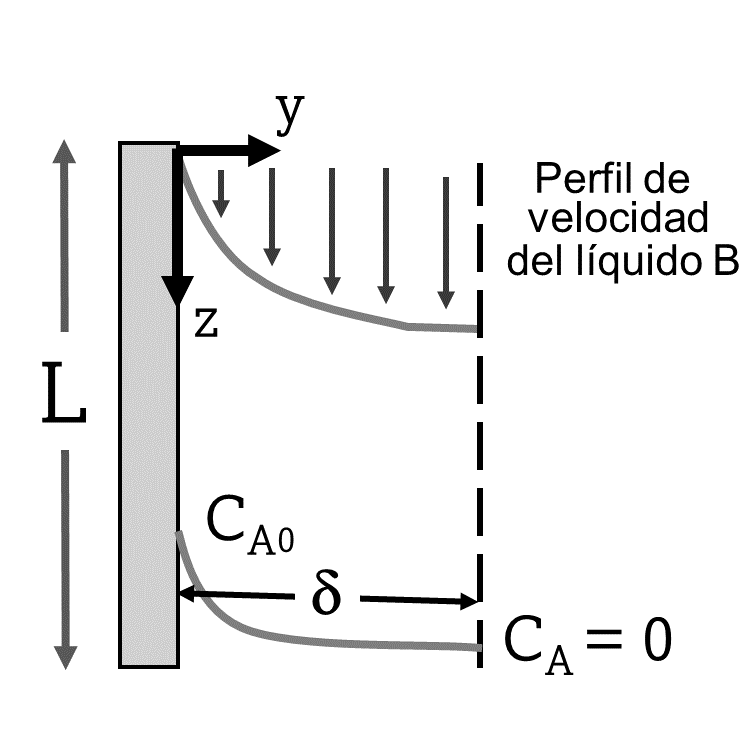
\includegraphics[scale=0.2]{./Capitulo2/Imagenes/fig-2-7.PNG}
	\caption{El sólido $A$ se disuelve en el líquido $B$ que desciende.}
\end{figure}

La concentración de $A$ en el líquido $B$ cambia dentro de una capa límite junto al sólido. El perfil de velocidades en una película descendente vertical, es:

\begin{equation}
	v_z = \frac{\rho g \delta^2}{2 \mu} \left[ 1 - \left( \frac{y'}{\delta} \right)^2 \right]
\end{equation}

En la aproximación de capa límite, se puede linealizar el perfil cerca de la pared, definiendo una variable $y$ de la forma: $y = \delta - y'$, de tal forma que: $1- \left( \frac{y'}{\delta} \right)^2 = 1 - \left( \frac{\delta - y}{\delta} \right)^2 = 1 - \left( 1- 2 \frac{y}{\delta} \right) =  \frac{2y}{\delta}$.  El perfil resultante es:

\begin{equation}
	v_z = \left( \frac{\rho g \delta}{\mu} \right) y = ay
\end{equation}

La ecuación de difusión en este caso es:

\begin{equation} \label{eq: manrefx10.1}
	ay \frac{\partial C_A}{\partial z} = \mathcal{D}_{AB} \frac{\partial^2 C_A}{\partial y^2}
\end{equation}

Las condiciones de frontera son:

\begin{equation}
	C_A|_{z=0} = 0
\end{equation}

\begin{equation}
	C_A|_{y=0} = C_{A0}
\end{equation}

\begin{equation}
	C_A|_{y \to \infty} = 0 \hspace{0.5cm} \text{(tiempo de contacto corto)}
\end{equation}

Por el método de combinación de variables, se sugiere la siguiente combinación:

\begin{equation} \label{eq: manrefx11}
	\frac{C_A}{C_{A0}} = f(\eta) \hspace{0.5cm} \text{donde} \hspace{0.5cm} \eta = y \left( \frac{a}{9 \mathcal{D}_{AB}z} \right)^{1/3}
\end{equation}

\begin{equation}
	\frac{\partial f}{\partial z} = \frac{\partial f}{\partial \eta} \left( \frac{\partial \eta}{\partial z} \right) = - y \left( \frac{a}{9 \mathcal{D}_{AB}} \right)^{1/3} \left( - \frac{1}{3} \frac{z^{-1/3}}{z} \right) = - \frac{1}{3} \frac{\eta}{z} \frac{d f}{d \eta}
\end{equation}

$$
\frac{\partial f}{\partial y} = \frac{\eta}{y} \frac{df}{d\eta} = \left( \frac{\partial \eta}{\partial y} \right) \frac{d f}{d \eta}
$$

\begin{equation} \label{eq: manrefx12}
	\frac{\partial^2 f}{\partial y^2} = \frac{\eta}{y} \frac{\partial \eta}{\partial y} \frac{d^2 f}{d y^2} = \frac{\eta^2}{y^2} \left( \frac{d^2 f}{d \eta^2} \right)
\end{equation}

Sustituyendo \eqref{eq: manrefx11} y \eqref{eq: manrefx12} en la ec. \eqref{eq: manrefx10.1} resulta en:

\begin{equation} \label{eq: manrefx13}
	\frac{d^2 f}{d \eta^2} + 3 \eta^2 \frac{df}{d \eta} = 0
\end{equation}

con condiciones de frontera:

\begin{equation} \label{eq: manrefx14}
	f|_{\eta = 0} = 1
\end{equation}

\begin{equation} \label{eq: manrefx15}
	f|_{\eta \to \infty} = 0
\end{equation}

La solución de \eqref{eq: manrefx13} es:

\begin{equation} \label{eq: manrefx16}
	f = C_1 \int_0^\eta e^{-\bar{\eta}^3} d \bar{\eta} + C_2
\end{equation}

La condición \eqref{eq: manrefx14} determina $C_2 = 1$. La condición \eqref{eq: manrefx15} determina \\ $C_1 = \dfrac{-1}{\int_0^\infty e^{-\bar{\eta}^3} d \bar{\eta}} = - \frac{1}{\Gamma (\frac{4}{3})}$ 

donde $\Gamma (x)$ es la función gamma de x. Como $\int_0^\eta = \int_0^\infty - \int_\eta^\infty$ entonces:

\begin{equation} \label{eq: manrefx16.1}
	\frac{C_A}{C_{A0}} = f =  \frac{\int_\eta^\infty e^{-\bar{\eta}^3} d\bar{\eta}}{\Gamma(\frac{4}{3})}
	\tag{\ref{eq: manrefx16}}
\end{equation}

\begin{equation}
	\begin{split}
	N_{Ay}|_{y=0} = - \mathcal{D}_{AB} \left.  \frac{\partial C_A}{\partial y} \right|_{y=0} = - \mathcal{D}_{AB} C_{A0} \left[ \frac{d}{d\eta} \left( \frac{C_A}{C_{A0}} \right) \frac{\partial \eta}{\partial y} \right]_{y=0} 
	\\
  = -\mathcal{D}_{AB} C_{A0} \left[ \frac{- e^{-\eta^3}}{\Gamma(\frac{4}{3})} \left( \frac{a}{9 \mathcal{D}_{AB}z} \right)^{1/3} \right]_{y=0} = \frac{\mathcal{D}_{AB} C_{A0}}{\Gamma (\frac{4}{3})} \left( \frac{a}{9 \mathcal{D}_{AB} z} \right)^{1/3}
	\end{split}
\end{equation}

El flujo molar de $A$ en $y=0$ es:

\begin{equation}
	\begin{split}
	W_A = \int_0^W \int_0^L N_{Ay}|_{y=0} dz dx
	=W \frac{\mathcal{D}_{AB} C_{A0}}{\Gamma(\frac{4}{3})} \left( \frac{a}{9 \mathcal{D}_{AB}} \right)^{1/3} \int_0^L z^{-1/3} dz \\
	=\left( \frac{3}{2} \right) \frac{\mathcal{D}_{AB} C_{A0} W}{\Gamma (\frac{4}{3})} \left( \frac{a}{9 \mathcal{D}_{AB}} \right)^{1/3} L^{2/3}
	=\frac{2 \mathcal{D}_{AB} C_{A0} WL}{\frac{4}{3} \Gamma (\frac{4}{3})} \left( \frac{a}{9 \mathcal{D}_{AB} L} \right)^{1/3}
	\end{split}
\end{equation}

donde $\frac{4}{3} \Gamma (\frac{4}{3}) = \Gamma (\frac{7}{3})$

\subsection{Perfil de concentración en un reactor tubular}

\begin{figure}[H]
	\centering
	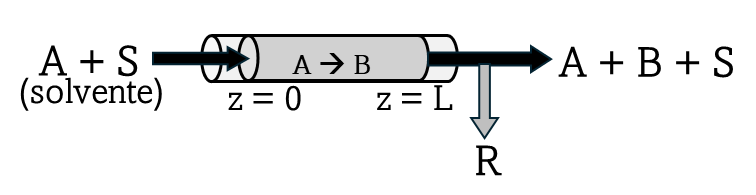
\includegraphics[scale=0.4]{./Capitulo2/Imagenes/fig-2-8.PNG}
	\caption{Reactor tubular}
\end{figure}

La situación es similar a las condiciones de la ec. \eqref{eq: manrefx2} en coordenadas cilíndricas, esto es: 

\begin{equation} \label{eq: manrefx17}
v_z \frac{\partial C_A}{\partial z} = \mathcal{D}_{AB} \left[ \frac{1}{r} \frac{\partial}{\partial r} \left( r \frac{\partial C_A}{\partial r} \right)  \right]
\end{equation}

\begin{equation} \label{eq: manrefx18}
\text{donde} \hspace{0.5cm} v_z = v_{z\text{máx}} \left[ 1 - \left( \frac{r}{R} \right)^2 \right]
\end{equation}

con condiciones:

\begin{equation}
C_A|_{z=0} = C_{A0} \hspace{0.2cm} , \hspace{0.2cm} C_A|_{r=R} = 0 \hspace{0.2cm} \text{y} \hspace{0.2cm} C_A|_{r=0} \neq 0
\end{equation}

La linealización del perfil de velocidades cerca de la pared procede definiendo una variable $y = R-r$:

Como $v_{\text{máx}} = \frac{\Delta P R^2}{2 \mu L}$, entonces $v_z (y) = v_{\text{máx}} \frac{y}{R} $

La ec. \eqref{eq: manrefx17} se transforma en:

\begin{equation}
	2 v_{\text{máx}} \frac{y}{R} = \mathcal{D}_{AB} \frac{\partial^2 C_A}{\partial y^2}
\end{equation}

debido a que $\frac{y}{R} = 1 - \frac{r}{R}$, entonces $\left( \frac{r}{R} \right)^2 = \left( 1 - \frac{y}{R} \right)^2 \approx 1 - \frac{2 y}{R} + \cdots$ por lo que $v_z = v_{z \text{máx}} (\frac{2y}{R})$ (ec. \eqref{eq: manrefx18}) con nuevas condiciones:

\begin{equation}
C_A|_{z=0} = C_{A0} \hspace{0.2cm} , \hspace{0.2cm} C_A|_{y=0} = 0 \hspace{0.2cm} \text{y} \hspace{0.2cm} C_A|_{y \to \infty} = C_{A0}
\end{equation}

La solución es similar a la ec. \eqref{eq: manrefx16.1}, excepto que ahora $f|_{\eta = 0} = 0$ y \\ $f|_{\eta \to \infty} = 1$. Las constantes son: $C_2 = 0$ y $C_1$ es igual: $C_1 = \frac{-1}{\Gamma (\frac{4}{3})}$, por lo tanto:

\begin{equation}
	\frac{C_A}{C_{A0}} = \frac{\int_0^\eta e^{- \bar{\eta}^3} d \bar{\eta}}{\Gamma (\frac{4}{3})}
\end{equation}
